\subsection{Внутреннее устойчивое множество}

Рассмотрим граф $G = (X, \Gamma)$, множество $S \subseteq V$ называется \textit{внутренне устойчивым}, если никакие две вершины из $S$ не смежны, другими словами если

\[
\Gamma S \cap S = \emptyset
\]

Обозначим через $\mathfrak{S}$ семейство всех внутренне устойчивых множеств графа; имеем

\[
S \in \mathfrak{S} \land S \subseteq A \Rightarrow A \in \mathfrak{S}
\]

По определению \textit{число внутренней устойчивости} графа $G$ есть

\[
\alpha(G) = \max_{S \in \mathfrak{S}} |S|
\]

\textbf{Замечание 1} Хроматическое число $\gamma(G)$ и число внутренней устойчивости $\alpha(G)$ связаны неравенством
\[
\alpha(G) \gamma(G) \geq |X|.
\]

В самом деле, можно разбить $X$ на $\gamma(G)$ внутренних устойчивых множеств, образованных вершинами одинакового цвета и содержащих соответственно $m_1, m_2, \ldots, m_q$ вершин. Поэтому
\[
|X| = m_1 + m_2 + \ldots + m_q \leq \gamma(G) \cdot \alpha(G) + \ldots + \alpha(G) = \gamma(G) \cdot \alpha(G).
\]

\textbf{Замечание 2} Можно поставить вопрос, не являются ли связи между обоими понятиями более тесными и нельзя ли найти хроматическое число, окрашивая сначала в цвет (1) наибольшее внутреннее устойчивое множество $S_1$, затем в цвет (2) наибольшее внутреннее устойчивое множество $S_2$ подграфа, порожденного вершинами $X \setminus S_1$, далее в цвет (3) наибольшее внутреннее устойчивое множество оставшегося подграфа и т.д. Оказывается, это не так, что видно на примере графа, изображенного на рис. 4--6 (его хроматическое число очевидно, равно 4), вершины, изображенные белыми кружками, образуют единственное наибольшее внутреннее устойчивое множество, но если их окрасить в один цвет, то остальные вершины $a \, b \, c \, d$ надо было бы окрасить с помощью только трех цветов, а это, очевидно, невозможно.

Иногда для двух графов $G$ и $H$ возникает вопрос о нахождении числа внутренней устойчивости произведения $G \times H$.

\begin{figure}[h]
    \centering
    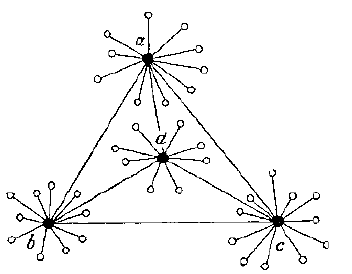
\includegraphics[width=0.5\textwidth]{example-imageю.png} % Replace with actual image path
    \caption{Рис. 4--6}
\end{figure}


\textbf{Лемма 1} Для двух графов $G$ и $H$
\[
\alpha(G \times H) \geq \alpha(G) \cdot \alpha(H)
\]

Действительно, если $S$ и $T$ — наибольшие внутренне устойчивые множества соответственно для $G$ и $H$, то декартово произведение $S \times T$ является внутренне устойчивым в графе $G \times H$, откуда
\[
\alpha(G \times H) \geq |S \times T| = |S| \cdot |T| = \alpha(G) \cdot \alpha(H)
\]

Эта лемма подсказывает нам следующее определение, назовем \emph{емкость} графа $G$ число
\[
\theta(G) = \sup_{n} \sqrt[n]{\alpha(G^n)}
\]

Имеем $\theta(G) \geq \alpha(G)$, мы собираемся показать, что почти всегда
\[
\theta(G) = \alpha(G)
\]

Между прочим, Шеннон установил, что граф $G$, изображенный на рис. 4-8, является единственным графом с числом вершин менее шести, для которого $\theta(G) \neq \alpha(G)$, фактически его емкость $\theta(G)$ не удалось определить, и известно лишь, что
\[
\forall \, 5 \leq \theta(G) \leq \frac{5}{2}
\]

Рассмотрим однозначное отображение $\sigma$ множества $X$ в себя, такое отображение называется \emph{сохраняющим}, если
\[
y \neq x, \, y \notin \Gamma(x) \Rightarrow \sigma(y) \neq \sigma(x), \, \sigma(y) \notin \Gamma(\sigma(x))
\]

Это отображение сохраняет свойство пары вершин "быть несмежными и различными".

\textbf{Лемма 2} Сохраняющее отображение $\sigma$ переводит внутренне устойчивое множество $S$ во внутренне устойчивое множество $\sigma(S)$, и при этом $|\sigma(S)| = |S|$.

В самом деле, ввиду однозначности отображения $\sigma$ имеем $|\sigma(S)| \leq |S|$, а так как $\sigma$ сохраняюще, то $|\sigma(S)| = |S|$.

\textbf{Лемма 3} Если множество $\sigma(X)$ внутренне устойчиво, то число внутренне устойчивости графа $G$ есть $\theta(G) = \alpha(G)$.

Действительно, раз $\sigma(X)$ внутренне устойчиво, то
\[
|\sigma(X)| \leq \max_{S} |S| = \alpha(G)
\]

С другой стороны, если $S_0$ — наибольшее внутренне устойчивое множество, то в силу леммы 2,

\[
|\sigma(X)| \geq |\sigma(S_0)| = |S_0| = \alpha(G),
\]

Отсюда

\[
\alpha(G) = |\sigma(X)|.
\]

\textbf{Теорема 7 (Шеннон)} \textit{Если хотя бы для одного из графов $G$ и $H$ существует сохранное отображение $\sigma$, переводящее множество вершин этого графа во внутренне устойчивое множество, то}

\[
\alpha(G \times H) = \alpha(G)\alpha(H).
\]

Достаточно показать, что $\alpha(G \times H) \leq \alpha(G)\alpha(H)$, пусть $\sigma$ — сохранное отображение для $G$, при котором $\sigma(X)$ внутренне устойчиво, и пусть $\sigma_0$ — отображение множества вершин графа $G \times H$ в себя, определенное следующим образом.

\[
\sigma_0(x, y) = (\sigma(x), y).
\]

Отображение $\sigma_0$ переводит две несмежные различные вершины $ξ = (x, y)$ и $ξ' = (x', y')$ в две несмежные различные вершины $(\sigma x, y)$ и $(\sigma x', y')$ и поэтому сохранно.

Если $S_0$ — наибольшее внутренне устойчивое множество графа $G \times H$, то $\alpha(G \times H) = |S_0| = |\sigma_0(S_0)|$ в силу леммы 2, распределим элементы $\sigma_0(S_0)$ по различным классам в зависимости от первой буквы каждого слова. Согласно лемме 3 получим: $|\sigma(X)| = \alpha(G)$ различных классов. Поскольку никакие два элемента из $\sigma_0(S_0)$ не смежны, каждый класс имеет самое большее $\alpha(H)$ элементов, значит

\[
\alpha(G \times H) = |\sigma_0(S_0)| \leq \alpha(G)\alpha(H).
\]

\textbf{Следствие} \textit{Если множество вершин графа $G$ при помощи сохранного отображения $\sigma$ можно перевести во внутренне устойчивое множество, то емкость этого графа совпадает с числом внутренней устойчивости.}

В самом деле,

\[
\alpha(G) \leq (\alpha(G))^2
\]

и

\[
\alpha(G \times G) \leq (\alpha(G))^3
\]

и т.д.,

отсюда

\[
\alpha(G) = \sup_n \sqrt[n]{\alpha(G^n)} = \alpha(G).
\]